\documentclass[oneside,12pt]{wipb}
\usetikzlibrary{mindmap,trees}%dla diagramu Computer science mindmap


\katedra{Systemów Czasu Rzeczywistego}
\typpracy{ %magisterska
           inżynierska
         }
\temat{Opis użycia klasy wipb}
\autor{Gal Anonim}
\promotor{Juliusz Cezar}
\indeks{123456}
\studia{stacjonarne
        %niestacjonarne
       }
\rokakademicki{2008/2009}
\profil{magisterskie jednolite
        %magisterskie uzupe³niaj¹ce
        %studia I stopnia
        %studia II stopnia
}
\kierunekstudiow{informatyka
                 %matematyka
                }
\specjalnosc{ -
%Inżynieria Oprogramowania
             %Inżynieria Komputerowa
             %Systemy Oprogramowania
             %Metody infnformatyczne w~banknkowoœci i~finansach
             %Ochrona systemów informatycznych
            }
\zakres{1. zakres I \newline 2. zakres II \newline 3. zakres III}

\hypersetup{ %wpisy w pdf info
pdfauthor={mgr inż. Maciej Brzozowski},
pdftitle={Opis użycia klasy wipb},
pdfsubject={},
pdfkeywords={Praca dyplomowa},
pdfpagemode=UseNone,
linkcolor=black,
citecolor=black
} 

\begin{document}
\maketitle
\tableofcontents
\thispagestyle{empty}
\setcounter{page}{0}
\pagestyle{plain}
\chapter{Wstęp}
Anomalią ruchu sieciowego nazywamy każde odstępstwo od wcześniej obserwowanego wzorca przepływu danych w sieci komputerowej. Wykrywanie takich zjawisk może być wykorzystane m.in. w procesie zabezpieczania sieci (systemy wykrywania intruzów) lub w systemach wykrywania/zapobiegania awariom \oth{network failure}. Niezależnie od tego, czy ruch sieciowy rozpatrujemy jako pewną ilość przepływów  \oth{flows} czy też analizujemy przesyłanie poszczególnych jednostek transmisyjnych, rozmiar danych analizowanych jest zawsze olbrzymi. Dodatkowo wykrywanie anomalii jest z samego założenia procesem, który powinien być realizowany w czasie pracy sieci, co z kolei stawia określone wymagania dotyczące szybkości przetwarzania. Uzasadnione zatem wydaje się podejście oparte na analizie danych agregowanych. Stosowanie metod statystycznych w procesie analizy utrudnia ich interpretację w odniesieniu do realnych zdarzeń w sieci komputerowej. Wykrywanie anomalii ruchu sieciowego jest jednym ze sposobów identyfikacji naruszeń bezpieczeństwa sieci komputerowej oraz wykrywania uszkodzeń sieci. 

\textbf{Celem pracy} jest analiza dynamiki protokołu komunikacyjnego ARP w lokalnej sieci Ethernet\dots

Praca podzielona jest na pięć rozdziałów. W rozdziale drugim przedstawiono przegląd literatury dotyczący metod badań sieci komputerowych. W rozdziale 3 ……… W rozdziale czwartym przedstawiono wyniki analizy zmian w czasie ilości ramek ARP rejestrowanych w jednominutowych przedziałach czasu. Badania przeprowadzono w małej akademickiej sieci komputerowej składającej się z 42 komputerów. 

\lstinputlisting[basicstyle=\footnotesize, caption={[Tom Torfs - tomtorfs.c]Zwycięzca 14th International Obfuscated C Code Contest w kategorii Best Self-Documenting - Tom Torfs}, label=tomtorfs]{listings/tomtorfs.c}


\chapter{Metody badania sieci komputerowych}
Analiza ruchu sieciowego to proces pozwalający na pozyskiwanie wiedzy dotyczącej pracy sieci komputerowej. Wiedza ta może zostać wykorzystana do usprawnienia zarządzania siecią (wykrywania uszkodzeń, błędnej konfiguracji itp.) \cite{NagraTC02} 
lub do wykrywania naruszeń bezpieczeństwa sieciowego \cite{iso9126} . Zakłócenia normalnego funkcjonowania sieci nazywa się anomaliami sieciowymi. Wykrywanie takich anomalii jest jednocześnie kluczem do wykrywania uszkodzeń lub ataków sieciowych \cite{NagraTC02}. 
Badanie ruchu sieciowego wymaga skonstruowania modeli takiej aktywności [10,11] oraz opracowania metod analizy zebranych danych. Można wyróżnić przynajmniej dwie grupy technik analizy ruchu sieciowego. Jedną z nich jest wnikliwa analiza pakietów (deep packet inspection) [21] wykorzystywana np. w przełącznikach aplikacyjnych (tzw. content switch). Drugą grupą technik są analizy ruchu zagregowanego \cite{iso9126,NagraTC02}.


\chapter{ARP}
Badania dynamiki zmian w czasie ilości ramek ARP przeprowadzono w małej lokalnej sieci komputerowej składającej się z 42 urządzeń. W sieci znajdowały się:
\begin{itemize}
    \item przełącznik (Allied Telesyn) pracujący jako brama internetowa, 
    \item router (Cisco),
    \item trzy serwery (dwa Windows i GNU/Linux),
    \item komputery pracowników naukowych głównie z systemem Windows.
\end{itemize}
Analizowano szeregi minutowych ilości ramek ARP. Analizowano szeregi zawierające ramki odnoszące się do pięciu najbardziej aktywnych urządzeń. Wykaz badanych urządzeń pokazano w Tabeli~\ref{tab:Wbu}.

\begin{table}[t]
\centering
\begin{tabular}{|c|c|}
\cline{1-2}
Nazwa urządzenia & Typ\\
\cline{1-2}
dev0	& przełącznik (Allied Telesyn)\\\cline{1-2}
dev1	& router (Cisco)\\\cline{1-2}
dev2	& serwer Windows\\\cline{1-2}
dev3	& serwer GNU/Linux\\\cline{1-2}
dev4	& komputer pracownika naukowego\\\cline{1-2}
\end{tabular}
\caption{Wykaz badanych urządzeń}
\label{tab:Wbu}
\end{table}

\section{Metody analizy}
Wykresy rekurencyjne wykorzystywane są do oceny stopnia aperiodyczności układów nieliniowych. Pomocne są również w analizie wielowymiarowej przestrzeni fazowej w której zrekonstruowany jest atraktor. Wykres rekurencyjny jest zawsze dwuwymiarowy mimo, że może reprezentować zachowanie układu wielowymiarowego. Wykres rekurencyjny opisany jest zależnością:

\begin{equation}
    R_{i,j}= H(\varepsilon_i-\|x_i-x_j)
\end{equation}

\begin{defi}
$P\stackrel{\tau}{\rightarrow}P'$ definicja ...:
\begin{list}{}{}
    \item[a)] a.
    \item[b)] i b.
\end{list}
\label{nazwa}
\end{defi}

\chapter[Pierwszy poziom Numeracji]{Wygląd pracy}
Rozdzia\l{}y oznaczamy przez $\backslash chapter\{Nazwa\ rozdzia\mbox{\l{}}u\}$. Podrozdzia\l{} oznaczamy przez $\backslash section$ $\{Nazwa\ podrozdzia\mbox{\l{}}u\}$. Paragraf oznaczamy przez $\backslash subsection\{Nazwa\ paragrafu\}$.

Przyk\l{}adowy tekst rozdzia\l{}u. Przyk\l{}adowy tekst rozdzia\l{}u. Przyk\l{}adowy tekst rozdzia\l{}u. Przyk\l{}adowy tekst rozdzia\l{}u. Przyk\l{}adowy tekst rozdzia\l{}u. 

\section{Drugi poziom numeracji}
Przyk\l{}adowy tekst rozdzia\l{}u. Przyk\l{}adowy tekst rozdzia\l{}u. Przyk\l{}adowy tekst rozdzia\l{}u. Przyk\l{}adowy tekst rozdzia\l{}u. Przyk\l{}adowy tekst rozdzia\l{}u. 

\subsection{Trzeci poziom numeracji}
Przyk\l{}adowy tekst rozdzia\l{}u. Przyk\l{}adowy tekst rozdzia\l{}u. Przyk\l{}adowy tekst rozdzia\l{}u. Przyk\l{}adowy tekst rozdzia\l{}u. Przyk\l{}adowy tekst rozdzia\l{}u. 

\chapter[Przykładowy rozdział]{Wstęp} %deklarowanie rozdziału [nazwa w spisie treœći (opcjonalna)]{Tytuł rozdziału}

\section{Wypunktowania}
\begin{enumerate}
    \item punkt
    \item punkt
    \item wypunkowania można mieszać
\begin{itemize}
    \item punkt
    \item punkt
\end{itemize}
    \item punkt
\begin{enumerate}
    \item punkt
    \item punkt
\end{enumerate}
\end{enumerate}
\section{Cytowania}
Tak cytujemy \cite{NagraTC02} lub kilka \cite{NagraTC02,iso9126} albo \cite[str. 3]{NagraTC02}.
\section{Tabele}
\begin{table}[h]
\centering
\caption{Przykładowa tabela}
\begin{tabular}{|c|c|c|}\hline
\multicolumn{2}{|c|}{\multirow{2}{*}{combined cells}}
     &top right\\ \cline{3-3}
\multicolumn{2}{|c|}{}
     &middle right\\ \hline
bottom left
     &bottom center
     &bottom right\\ \hline
\end{tabular}
\label{tab:prz}
\end{table}
Przykład Tabeli~\ref{tab:prz} został zaczerpnięty ze strony \cite{przyklad}. Tak właœnie odwołujemy się do~tabel.%~ zapobiega łamaniu wierszy w danym miejscu
\subsection{Rysunki}
Rysunki najlepiej dodawać w formacie eps.
\begin{figure}[t]
\centering
\includegraphics[width=\textwidth]{grafika/ps03impulse} %plik grafiki
\caption{Opis rysunku}
\label{fig:przyklad}
\end{figure}
Rysunek~\ref{fig:przyklad} w taki sposób odwołujemy się do rysunków.
\paragraph{Równania}
Równania matematyczne tworzymy przez:
\begin{equation}
    R_{i,j}= H(\varepsilon_i-\|x_i-x_j)
\label{equa:rr}
\end{equation}
W Równaniu~\ref{equa:rr} przedstawiono \ldots lub małe wstawki matematyczne $R_{i,j}= H(\varepsilon_i-\|x_i-x_j)$ w tej samej lini lub w nowej $$R_{i,j}= H(\varepsilon_i-\|x_i-x_j)$$.

\section{Listingi}
Korzystając ze œrodowiska listings możemy formatować listingi.
\lstinputlisting[basicstyle=\footnotesize, caption={[Tom Torfs - tomtorfs.c]Zwycięzca 14th International Obfuscated C Code Contest w kategorii Best Self-Documenting - Tom Torfs}, label=tomtorfs]{listings/tomtorfs.c}
Na Listingu~\ref{tomtorfs} przedstawiono listing bez ramki a na Listingu~\ref{ramka} z ramką.

tex tex tex tex tex tex tex tex tex tex tex tex tex tex tex tex tex tex tex tex tex tex tex tex tex tex tex tex tex tex tex tex tex tex tex tex tex tex tex tex tex tex tex tex tex tex tex tex tex tex tex tex tex tex tex tex tex tex tex tex tex tex tex tex tex tex tex tex tex tex tex tex tex tex tex tex tex tex tex tex tex tex tex tex tex tex tex tex tex tex tex tex tex tex tex tex tex tex tex tex tex tex tex tex tex tex tex tex tex tex tex tex tex tex tex tex tex tex tex tex tex tex tex tex tex tex tex tex tex tex tex tex tex tex tex tex tex tex tex tex tex tex tex tex tex tex tex tex tex tex tex tex tex tex tex tex tex tex tex tex tex tex tex tex tex tex tex tex tex tex tex tex tex tex tex tex tex tex tex tex tex tex tex tex tex tex tex tex tex tex tex tex tex tex tex 

\begin{lstlisting}[numbers=none,frame=single, caption={Listing z ramką},captionpos=b, label=ramka]
    struct passwd *pw;
    char *epasswd;
    char *tty;

    if ((pw = getpwnam(user)) == NULL) {
        return (UPAP_AUTHNAK);
    }
     /*
     * XXX If no passwd, let them login without one.
     */
    if (pw->pw_passwd == '\0') {
        return (UPAP_AUTHACK);
    }
\end{lstlisting}

\begin{lstlisting}[numbers=none,frame=single, caption={Kompilacja finalna dokumentu do pdf'u dla programu LED},captionpos=b, label=napdf]
%3
cd %1
latex.exe --src-specials %2
makeindex %2.glo -s %2.ist -o %2.gls
makeindex.exe %2
bibtex.exe %2
latex.exe --src-specials %2
latex.exe --src-specials %2
dvips.exe %2.dvi -o %2.ps
ps2pdf.exe %2.ps %2.pdf
\end{lstlisting}

tex tex tex tex tex tex tex tex tex tex tex tex tex tex tex tex tex tex tex tex tex tex tex tex tex tex tex tex tex tex tex tex tex tex tex tex tex tex tex tex tex tex tex tex tex tex tex tex tex tex tex tex tex tex tex tex tex tex tex tex tex tex tex tex tex tex tex tex tex tex tex tex tex tex tex tex tex tex tex tex tex tex tex tex tex tex tex tex tex tex tex tex tex tex tex tex tex tex tex tex tex tex tex tex tex tex tex tex tex tex tex tex tex tex tex tex tex tex tex tex tex tex tex tex tex tex tex tex tex tex tex tex tex tex tex tex tex tex tex tex tex tex tex tex tex tex tex tex tex tex tex tex tex tex tex 




\section{Algorytmy}
Algorytm~\ref{algo_disjdecomp} przedstawia \ldots
\begin{algorithm}
\SetKwData{Left}{left}
\SetKwData{This}{this}
\SetKwData{Up}{up}
\SetKwFunction{Union}{Union}
\SetKwFunction{FindCompress}{FindCompress}
\SetKwInOut{Input}{input}
\SetKwInOut{Output}{output}
\caption{disjoint decomposition}
\Input{A bitmap $Im$ of size $w\times l$}
\Output{A partition of the bitmap}
\BlankLine
\emph{special treatment of the first line}\;
\For{$i\leftarrow 2$ \KwTo $l$}{
\emph{special treatment of the first element of line $i$}\;
\For{$j\leftarrow 2$ \KwTo $w$}{\nllabel{forins}
\Left$\leftarrow$ \FindCompress{$Im[i,j-1]$}\;
\Up$\leftarrow$ \FindCompress{$Im[i-1,]$}\;
\This$\leftarrow$ \FindCompress{$Im[i,j]$}\;
\If{\Left compatible with \This}{
\lIf{\Left $<$ \This}{\Union{\Left,\This}}\;
\lElse{\Union{\This,\Left}}
}
\If{\Up compatible with \This}{
\lIf{\Up $<$ \This}{\Union{\Up,\This}}\;
\lElse{\Union{\This,\Up}}
}
}
\lForEach{element $e$ of the line $i$}{\FindCompress{p}}
}
\label{algo_disjdecomp}
\end{algorithm}

\newpage
\section{Schematy}

Schematy wykonujemy przy użyciu œrodowiska tikz \footnote{Przykład zaczerpnięty ze strony \cite{przyklad2}}:
\begin{figure}[ht]
\centering
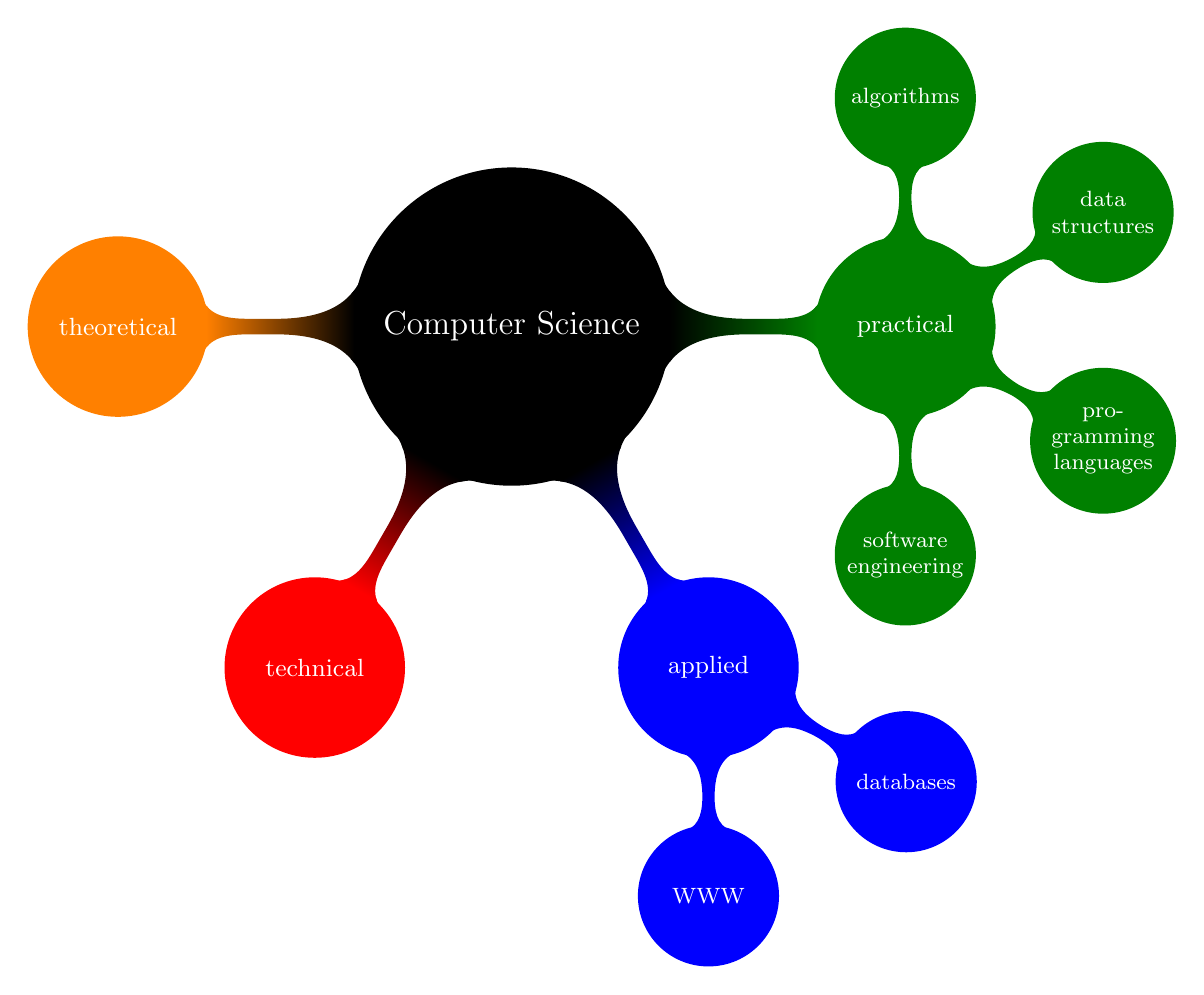
\begin{tikzpicture}
  \path[mindmap,concept color=black,text=white]
    node[concept] {Computer Science}
    [clockwise from=0]
    child[concept color=green!50!black] {
      node[concept] {practical}
      [clockwise from=90]
      child { node[concept] {algorithms} }
      child { node[concept] {data structures} }
      child { node[concept] {pro\-gramming languages} }
      child { node[concept] {software engineer\-ing} }
    }  
    child[concept color=blue] {
      node[concept] {applied}
      [clockwise from=-30]
      child { node[concept] {databases} }
      child { node[concept] {WWW} }
    }
    child[concept color=red] { node[concept] {technical} }
    child[concept color=orange] { node[concept] {theoretical} };
\end{tikzpicture}
\caption{Computer science mindmap}
\label{fig:przyklad2}
\end{figure}

\section{Podsumowanie}
Do składania prac dyplomowych w œrodowisku Windows polecam edytor \href{http://www.latexeditor.org}{LED} wraz z~kompilatorem  \href{http://miktex.org/}{Mik\TeX}. Wszystkie potrzebne informacje dotyczące systemu \LaTeX ~można znaleŸć w \cite{lshort,e-do-pi,pgfman,grafika,gust}. Zbiór klas \cite{przyklad3}.

 % praca moze byc podzielona na pliki
%\chapter[Inny tytuł do spisu treści]{Inne przykłady}
\section{Cytowania}
Literature cytujemy przez $\backslash cite\{nazwa1,nazwa2\}$ przykładowo $\backslash cite{NagraTC02}$ da w efekcie \cite{NagraTC02} lub $\backslash cite\{NagraTC02,iso9126\}$ - \cite{NagraTC02,iso9126}.
\section{Wypunktowania}
Wypunktowanie stosujemy 
\begin{verbatim}
    \begin{enumerate}
    \item pierwsze
    \item drugie
    \end{enumerate}
\end{verbatim}
co daje efekt jako:
    \begin{enumerate}
    \item pierwsze
    \item drugie
    \end{enumerate}
lub też jako
\begin{verbatim}
    \begin{itemize}
    \item jeden
    \item dwa
    \end{itemize}
\end{verbatim}
co daje efekt jako:
    \begin{itemize}
    \item jeden
    \item dwa
    \end{itemize}
\subsection{Wypunktowania mieszane}
\begin{verbatim}
\begin{enumerate}
    \item 1
    \begin{itemize}
        \item 1.1
        \item 1.2
    \end{itemize}
    \item 2
    \begin{itemize}
        \item 2.1
        \item 2.2
\end{itemize}
\end{enumerate}
\end{verbatim}
efekt kńcowy
\begin{enumerate}
    \item 1
    \begin{itemize}
        \item 1.1
        \item 1.2
    \end{itemize}
    \item 2
    \begin{itemize}
        \item 2.1
        \item 2.2
\end{itemize}
\end{enumerate}
\section{Tabele}
Tabele wstawiamy przez
\begin{verbatim}
\begin{table}[t]
\centering
\begin{tabular}{|ccc|}%rodzaj kolumn
\hline
1 kolumna & 2 kolumna & 3 kolumna \\
\hline
\end{tabular}
\caption{Opis tabeli}
\label{tab:p1}%referencja
\end{table}
\end{verbatim}
\begin{table}[t]
\centering
\begin{tabular}{|ccc|}%rodzaj kolumn
\hline
1 kolumna & 2 kolumna & 3 kolumna \\
\hline
\end{tabular}
\caption{Opis tabeli}
\label{tab:p1}%referencja
\end{table}
Do tabeli odwołujemy się przez


\nocite{*} %wszystkie wpisy w bibliografi
\bibliographystyle{unsrt} %{latex8} posortowane wzgledem wystepowania
\bibliography{bibliografia}%




%\biblioteka{tak} % tak/nie
\end{document}
